\chapter{Analysis of Collected Data}
\label{chap:analysis}

\itquote[0mm]{
The goal is to turn data into information, and information into insight.
}{C. Fiorina}

In order to get insight into how the deployed system works
and what should we focus on in next iterations,
we analyze collected data.
All analyses in this chapter use data collected  % avoid repeating "collected"
during 4 months (10th November 2017 -- 9th March 2018).
This data, as well as the code performing the analyses, are available
as attachments of this thesis
(described in \cref{sec:attachment.collected-data,sec:attachment.analyses}).


\section{Data Description}

During the 4 months, about 1000 users tackled at least one task,
%\footnote{The true number of unique users might be lower, because a single user
%may be counted multiple times if he had not signed up and used the system again
%after a session cookie had expired. However, the Google Analytics suggests
%that the number is approximately correct.},
and 800 of them solved at least one task.
About 100 students returned and solved another task another day.
\Cref{fig:engagement-curves} shows complete engagement curves.
% TODO (GA):
Nearly all users access the webpage on a desktop computer ($94\%$).
% TODO: and does any of the mobile-users solved any task? (because that would be very difficult)
% Desktop 94%, Mobile 4%, Tablet 2%

\begin{figure}[htb]
\centering
\begin{subfigure}{.49\textwidth}
\centering
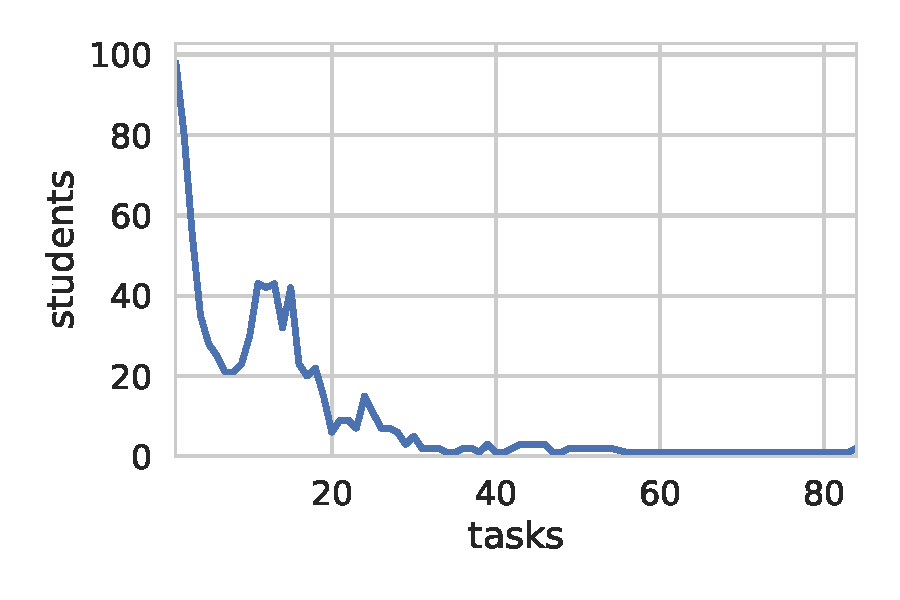
\includegraphics[height=42mm]{img/engagement-tasks}
%\caption{How many students solved given number of tasks.}
\end{subfigure}
\begin{subfigure}{.49\textwidth}
\centering
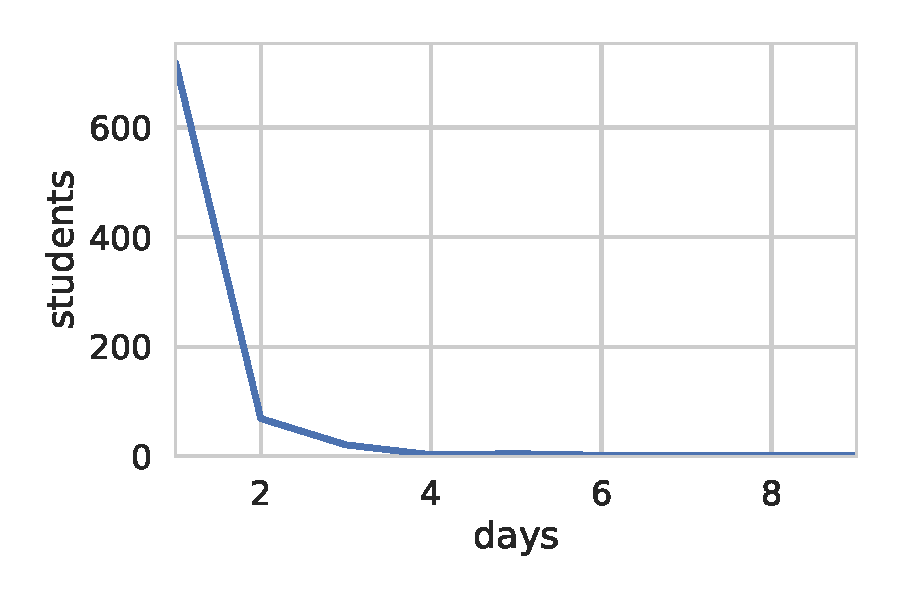
\includegraphics[height=42mm]{img/engagement-days}
%\caption{How many students solved a task given number of days.}
\end{subfigure}
\caption{%
  Engagement curves show how many students solved at least given number of task (left),
  and how many students solved a task at least given number of days (right).}
\label{fig:engagement-curves}
\end{figure}


About 11000 tasks were attempted (counting only those attempts with at least one edit),
and 9600 of them were solved,
resulting in the overall success rate $86\%$.
The daily numbers of solved task sessions are not stable,
with high peaks on days when the application was used
in a competition or testing at a school
(\cref{fig:daily-task-sessions}).
% The following can be a separate paragraph, if another
% analysis is performed.
Over 180 thousand program snapshots was collected,
from which 140 thousand corresponds to edits,
and 40 thousand to executions.

% TODO: join with another plot (-> two plots on a single line).
% (e.g. a metric mentioned at the theory part)
% TODO: crop/tighten margings (esp. the bottom one)
%\imgW[0.3]{daily-task-sessions}{%
%  Daily number of solved task sessions (weekly averaged).}
\begin{figure}[htb]
\centering
%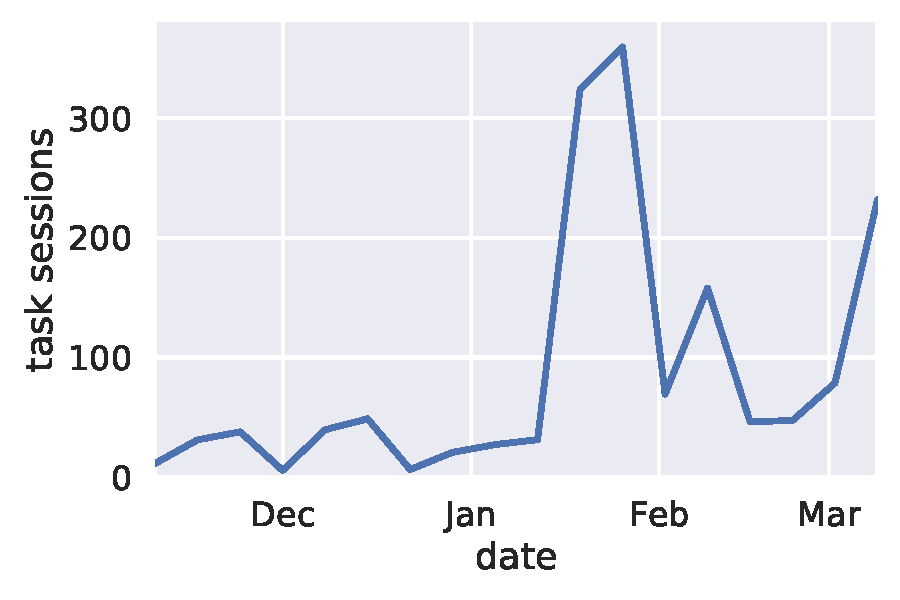
\includegraphics[width=0.48\textwidth,trim={0 21mm 0 7mm},clip]{img/daily-task-sessions}
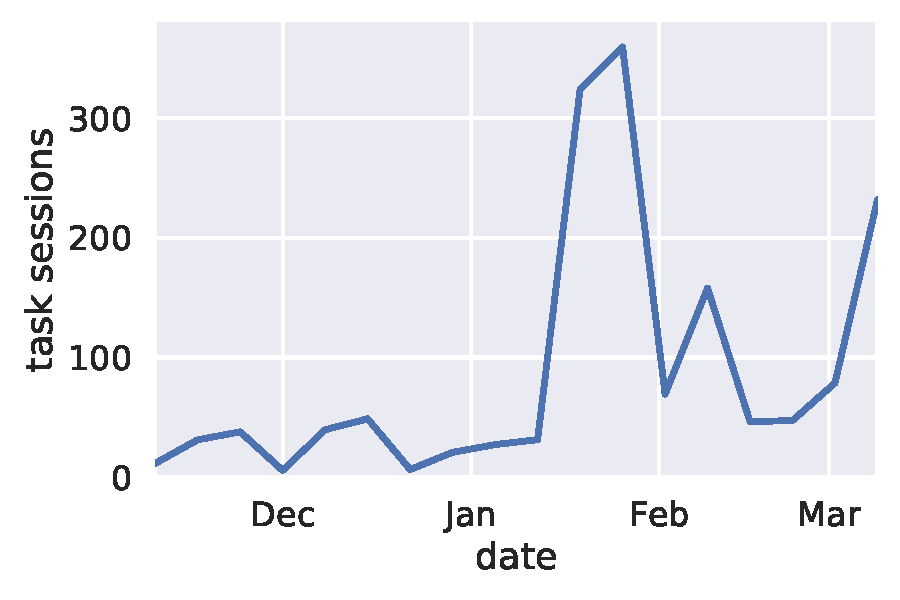
\includegraphics[width=0.48\textwidth]{img/daily-task-sessions}
\caption{Daily number of solved task sessions (weekly averaged).}
\label{fig:daily-task-sessions}
\end{figure}

Median solving time is 1 minute (interquartile range: 24--145 seconds).
Solving times follow log-normal distribution (\cref{fig:solving-times}),
so the mean solving time is much higher
(about 3 minutes). %195 seconds, % with high standard deviation of nearly 500 seconds.
% even if the times are capped at one hour).
% and not very informative


\begin{figure}[htb]
\centering
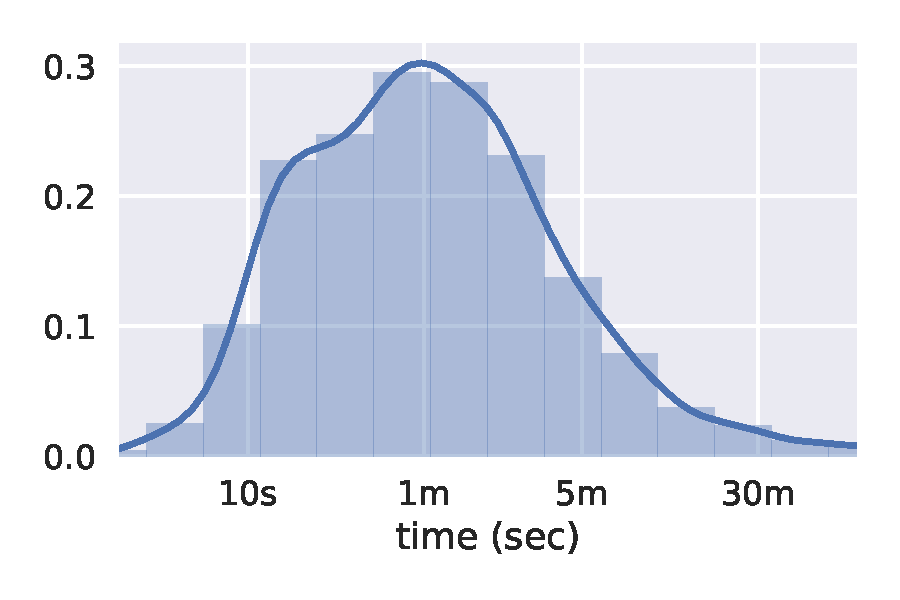
\includegraphics[width=0.48\textwidth]{img/task-sessions-time-log}
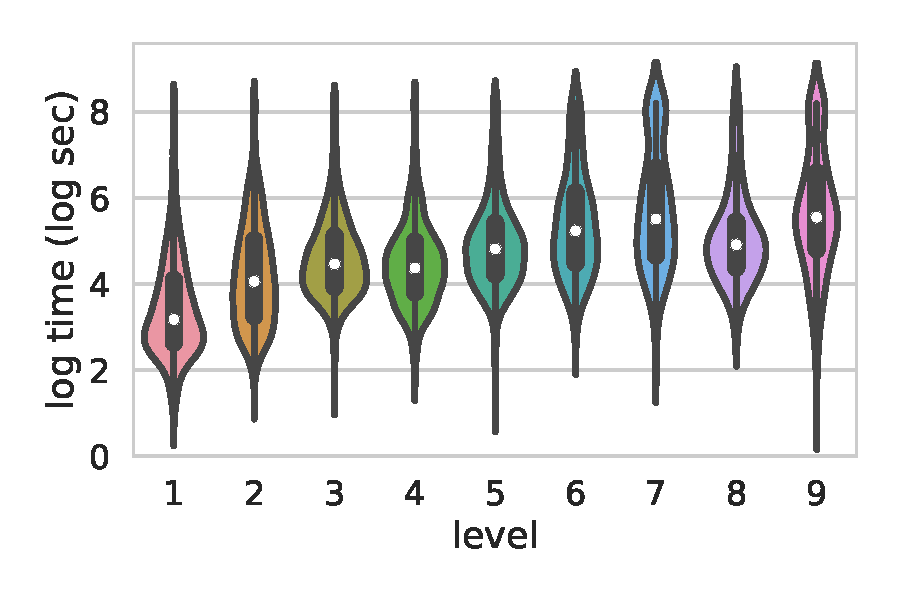
\includegraphics[width=0.48\textwidth]{img/levels-time}
\caption{%
  Distribution of log-transformed solving times.
  Left: All task sessions.
  Right: For each level.}
\label{fig:solving-times}
\end{figure}

\section{Behavior Evaluation}

Checking the requirements mentioned in: \cref{sec:robomission.behavior}.

Progress to 2nd level:
73\% of students who are still learning after 10 minutes has reached 2nd level at that time
\cref{fig:students-at-levels}.

\begin{figure}[htb]
\centering
\begin{subfigure}{.49\textwidth}
\centering
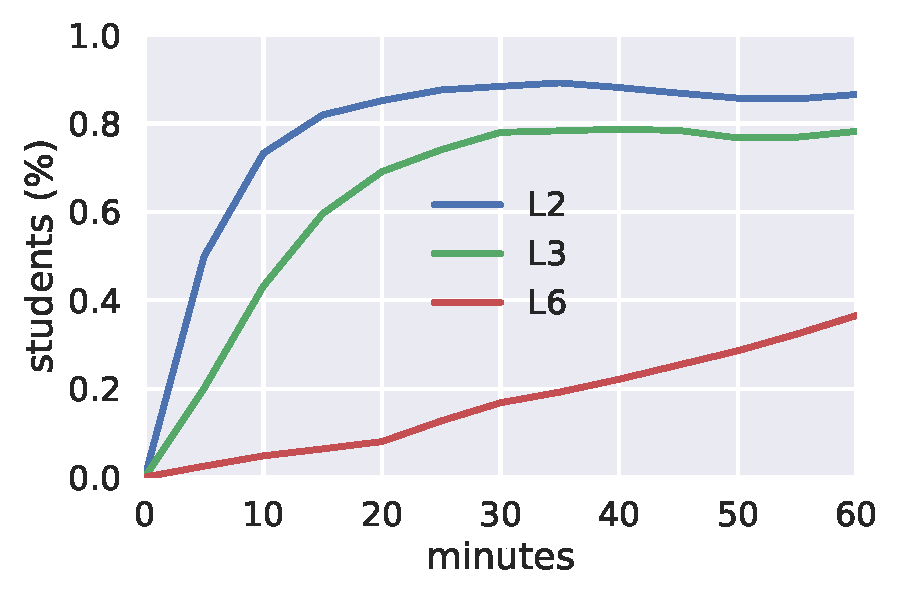
\includegraphics[height=42mm]{img/students-at-levels}
%\caption{How many students solved given number of tasks.}
\end{subfigure}
\begin{subfigure}{.49\textwidth}
\centering
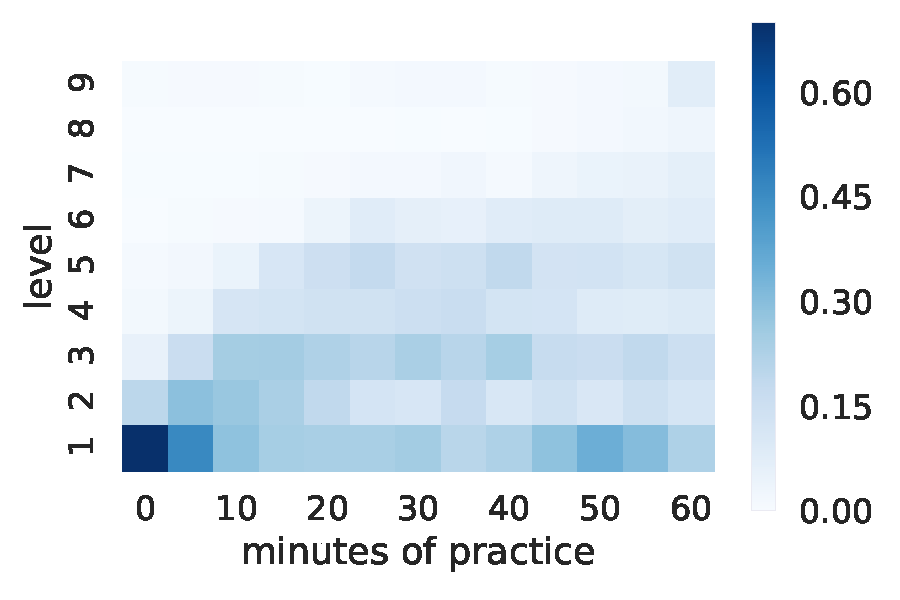
\includegraphics[height=42mm]{img/task-sessions-at-levels}
%\caption{How many students solved a task given number of days.}
\end{subfigure}
\caption{%
  Left: proportion of students in the system after some time of practicing,
  who progressed to the 2nd, 3rd, and 6th level (sequence of commands, repeat loop, if-statements).
  Right: how the proportion of tasks at different levels is shifting during the practice.}
\label{fig:students-at-levels}
\end{figure}

\section{Performance Compression}

% In ... we have discussed importance of a performance compression
Our student model uses three-valued performance representation, and
a performance compression function based purely on observed solving time
(\cref{sec:robomission.student}).
Would using other observational data, such as number of edits
bring more information about the performance?
(TODO: Goal: find a compression function that maximizes performance of
student model.)

Overall Pearson correlation between solving times and number of edits (both
log-transformed) is quite high (0.73). However, if computed for individual tasks,
median correlation drops to 0.64, % (interquartile range 0.5 -- 0.72),
and $25\%$ of tasks have a correlation below 0.5 % check the number
(\cref{fig:time-vs-edits}), which suggests that incorporating number of edits
(or executions) should be at least considered.


\begin{figure}[htb]
\centering
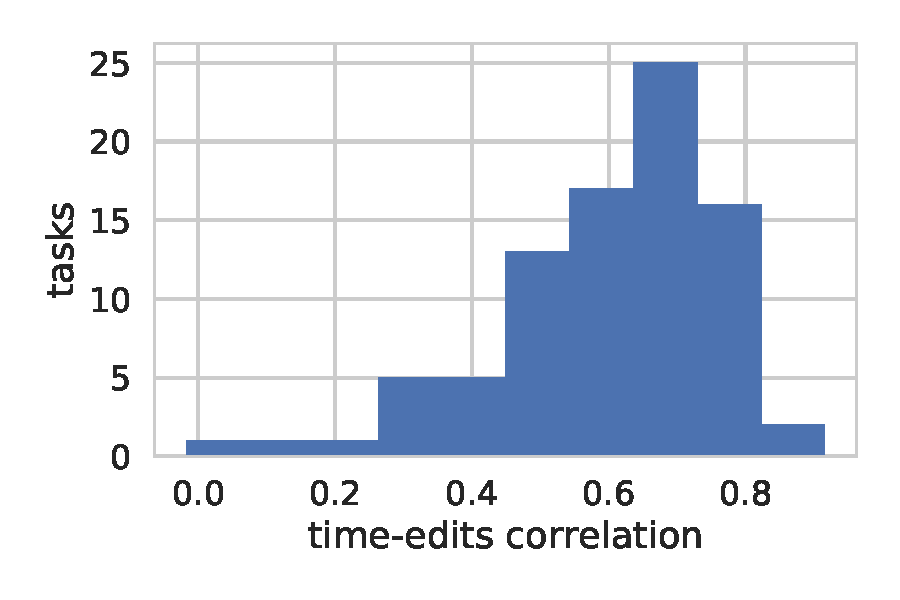
\includegraphics[width=0.48\textwidth]{img/time-edits-corr}
%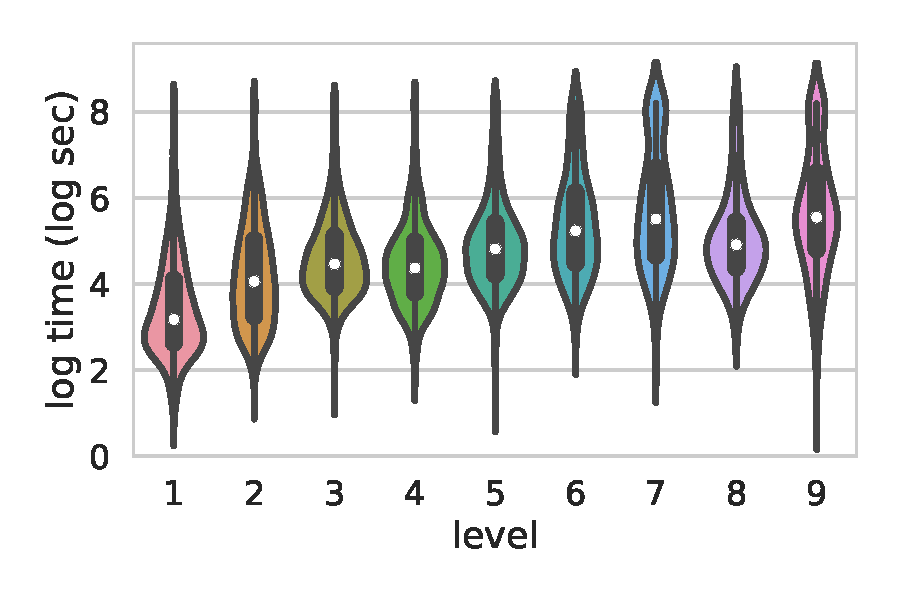
\includegraphics[width=0.48\textwidth]{img/levels-time}
\caption{%
  Distribution of Pearson correlations between median solving times and number
  of edits (both log-transformed) for individual tasks.} %  TODO: another plot on the right.}
\label{fig:time-vs-edits}
\end{figure}


\section{Task Difficulties}

% Reformulate to make it clear, that it is the analysis before introduction of the phases,
% that actually leads to the refinement described in the thesis.

% TODO: Resolve mission vs. level.
Our tutor model (\cref{robomission.tutor}) assumes that difficulties of tasks
in each phase are approximately the same,
and that the overall difficulty is increasing as the level increases.   % even phase.
Using collected data, we can determine whether these assumption are satisifed,
and if not, suggest adjustments to improve their validity.

\Cref{fig:solving-times} (right) shows that on average the difficulty of levels
is increasing, but it also reveals that level 7 is more difficult than level 8.
% TODO: Elaborate on the solution to this issue.
% (TODO?: phases instead of missions, and select only a few to save space)
Looking at the difficulty of individual tasks (\cref{fig:difficulties-tasks-levels})
help us to discover outliers, whose difficulty is significantly
different from the other tasks in the same level.
The \cref{fig:difficulties-tasks-levels} also suggests that dividing levels
into phases is necessary to achieve reasonable homogenity. For example, in the 2nd
level (World), there are two clear groups of tasks with significantly different
difficulty. Although in the other levels such a clear split does not exist,
they still often contain tasks with a wide range of difficulties.
% TODO: note/analyze robustness of these analyses (given the limited data)

\begin{figure}[htb]
\centering
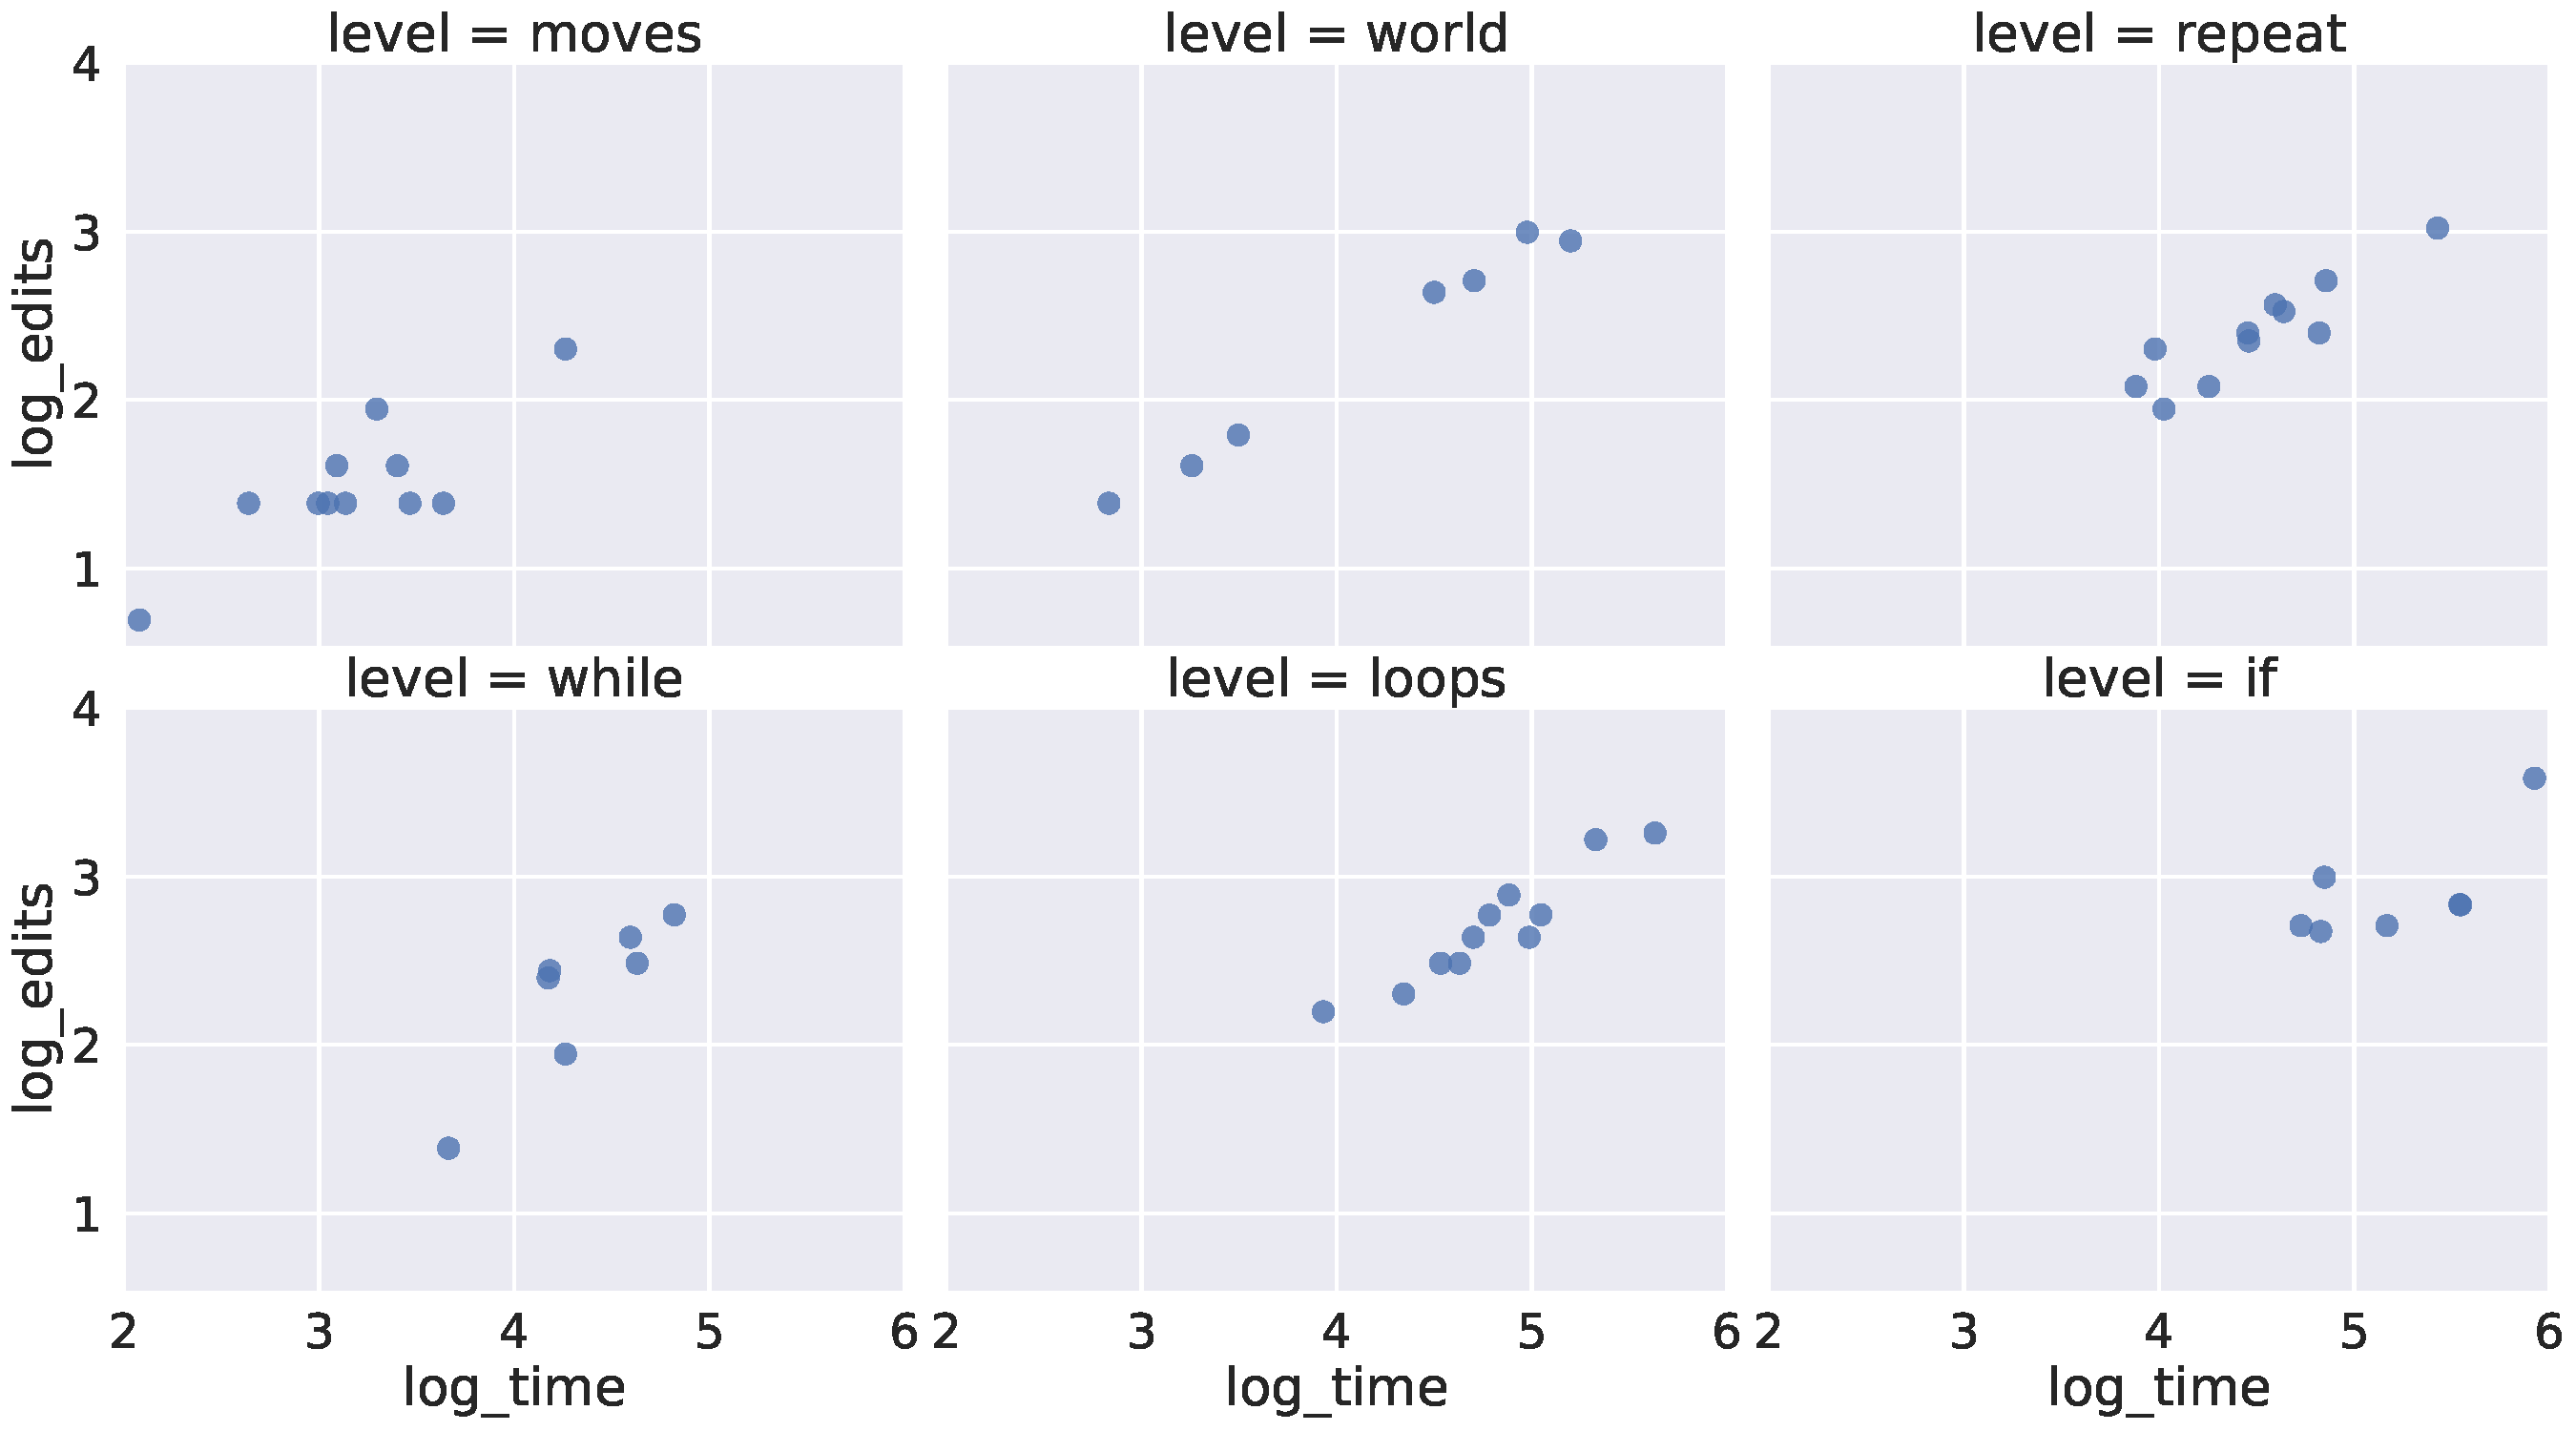
\includegraphics[width=\textwidth]{img/difficulties-tasks-levels}
\caption{%
  Difficulties of tasks in the first 6 levels.
  Difficulty is measured as spent time and number of edits, both log-transformed.}
\label{fig:difficulties-tasks-levels}
\end{figure}

%\imgW{difficulties-tasks-levels}{%
%  Difficulties (spent times and number of edits, both log-transformed)
%  of tasks in each level.}
